\section{Experimentación}

Respecto a la experimentación, el software para balancear las clases está implementado en Python mientras que las ejecuciones experimentales se han realizado en JCLEC.

% TODO: Explicar el algoritmo de Bojarczuk_GP


\newpage

\subsection{Validación de las pruebas}


Uno de los problemas que nos encontramos en los algoritmos de aprendizaje automático es la validación del algoritmo, es decir, como podemos asegurar que nuestro algoritmo realmente funciona, y no se trata de que ha hecho un sobreajuste con los datos con los que ha entrenado y fuera de dichos datos no es capaz de realizar buenas predicciones.

Para comprobar y asegurarnos que los algoritmos son capaces de realizar buenas predicciones fuera de los datos con los que ha entrenado utilizaremos validación cruzada con $k$ iteraciones.

Este método consiste en dividir el conjunto de entrenamiento en $k$ partes de mismo tamaño, de forma que realizaremos $k$ iteraciones para entrenar nuestro modelo. En cada iteración utilizaremos una de estas partes como conjunto de validación y las otras $k - 1$ partes como conjunto de entrenamiento, de forma que el algoritmo no haya entrenado con esa parte de validación. Finalmente para obtener el error del algoritmo para dicho conjunto de datos utilizaremos la media del error en los distintos conjuntos de validación de cada iteración.

Es importante destacar que antes de hacer las separaciones en $k$ subconjuntos de datos el conjunto de entrenamiento se reordenará de forma aleatoria para evitar que un conjunto en el que los datos estén ordenados por clase se excluya del entrenamiento cierta clase, porque todas sus muestras están en el conjunto de validación.

De esta forma podremos obtener un valor del error del algoritmo para unos datos con los que no ha entrenado, a la vez que comprobamos que nuestro algoritmo es capaz de ajustarse bien o no a un conjunto de datos.


\begin{figure}[H]
    \centering

	 \begin{subfigure}[b]{\textwidth}
		\centering
		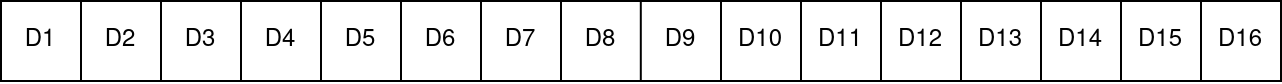
\includegraphics[width=0.8\textwidth]{cross_validation/conjunto_datos.png}
		\caption{Ejemplo de un conjunto de 16 datos.}
	  \label{fig:ej_16_datos}
   \end{subfigure}
	\vspace{1cm}

	 \begin{subfigure}[b]{\textwidth}
		 \centering
		 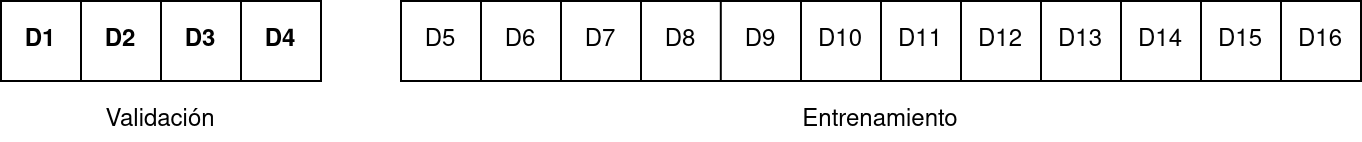
\includegraphics[width=0.8\textwidth]{cross_validation/iteracion1.png}
 		 \caption{Separación entre validación y entrenamiento en la primera iteración.}
 	    \label{fig:cv_iteracion1}
	 \end{subfigure}
	 \vspace{1cm}

	\begin{subfigure}[b]{\textwidth}
		 \centering
		 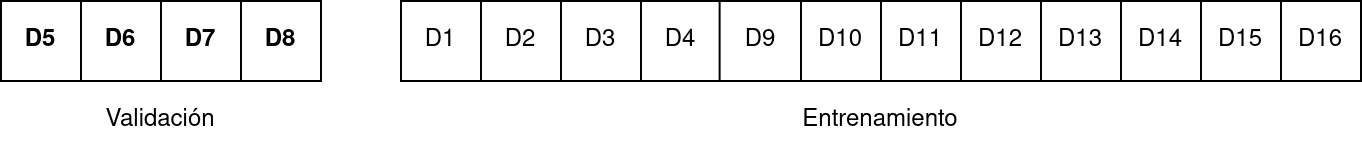
\includegraphics[width=0.8\textwidth]{cross_validation/iteracion2.png}
 		 \caption{Separación entre validación y entrenamiento en la segunda iteración.}
 	    \label{fig:cv_iteracion2}
   \end{subfigure}
	\vspace{1cm}

	\begin{subfigure}[b]{\textwidth}
		 \centering
		 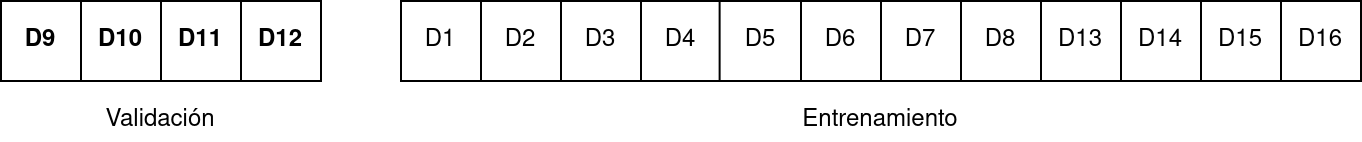
\includegraphics[width=0.8\textwidth]{cross_validation/iteracion3.png}
 		 \caption{Separación entre validación y entrenamiento en la tercera iteración.}
 	    \label{fig:cv_iteracion3}
	\end{subfigure}
	\vspace{1cm}

	\begin{subfigure}[b]{\textwidth}
		 \centering
		 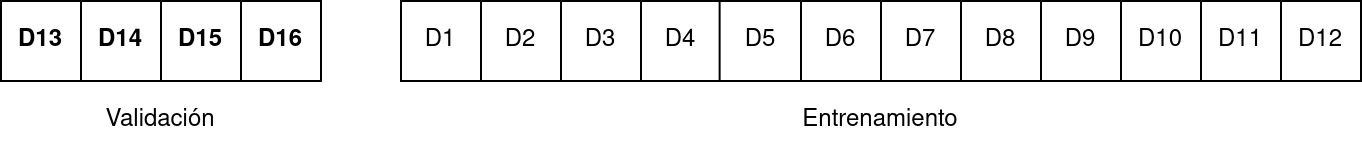
\includegraphics[width=0.8\textwidth]{cross_validation/iteracion4.png}
 		 \caption{Separación entre validación y entrenamiento en la cuarta iteración.}
 	    \label{fig:cv_iteracion4}
	\end{subfigure}

	\caption{Ejemplo de validación cruzada de 4 iteraciones.}
	\label{fig:4-cv-ejemplo}
\end{figure}


\subsubsection{Validación cruzada utilizando 5x2cv}

En nuestro caso utilizaremos 5x2cv para validación. Este método fue propuesto por Thomas G. Dietterich en el año 1998 \cite{propuesta5x2cv}.

Este método se basa en realizar cinco repeticiones de una validación cruzada con dos iteraciones, cada una de estas repeticiones utilizando particiones distintas de los datos al 50\%. De esta forma, con cada una de las cinco particiones que realicemos a los datos aplicaremos una validación cruzada con dos folds, entrenando con la primera mitad de los datos y validando con la segunda mitad en el primer fold, y al contrario en el segundo fold.

Como podemos ver, con cinco repeticiones y siendo cada una de estas un 2-cv (de ahí el nombre 5x2cv) obtendremos diez valores de error, siendo el error final obtenido en validación la media de estos diez valores.



\newpage

\subsection{Funciones de evaluación}

De cara a evaluar los algoritmos necesitaremos una función de evaluación que nos permita saber el error que estamos cometiendo en las estimaciones.

En nuestro caso, al estar ante un problema de clasificación utilizaremos las siguientes:

\begin{itemize}
	\item Precisión.
	\item Área bajo la curva ROC.
	\item Error absoluto medio ordinal.
\end{itemize}

\subsubsection{Precisión}


\subsubsection{Área bajo la curva ROC}


\subsubsection{Error absoluto medio ordinal}



\newpage
